\documentclass{beamer}
\usepackage{graphicx}
\usepackage{amsmath}

\title{Monetary and Fiscal Policy Analysis --- December 16, 2008}
\author{Anuj Patel, Charles Ancel, and Henry Szklanny (Team Two)}
\date{August 2nd, 2024}

\begin{document}

\frame{\titlepage}

\section{Contextual Information}
\begin{frame}
    \frametitle{Contextual Information}
    \begin{itemize}
        \item FOMC lowered federal funds rate by 50 basis points to 1\% due to slowing economic activity.
        \item National Bureau of Economic Research declared recession on December 1st\@.
        \item Declines in retail sales, manufacturing, real estate, and lending.
        \item Weakened labor markets, decreased price pressures, and further financial market declines.
        \item Projected 5\% GDP fall over the next two quarters.
        \item Unemployment rising to 8\% in 2010.
        \item PCE inflation around 1\% for 2009 and 2010.
    \end{itemize}
\end{frame}

\section{Contextual Data}
\begin{frame}
    \frametitle{Contextual Data --- GDP}
    \begin{itemize}
        \item GDP from Q4 2003 to Q4 2013.
        \item Recession period.
        \item Q4 2008 GDP\@: approximately 14.608 trillion USD\@.
    \end{itemize}
\end{frame}

\begin{frame}
    \frametitle{Graph --- GDP}
    \begin{figure}[h!]
        \centering
        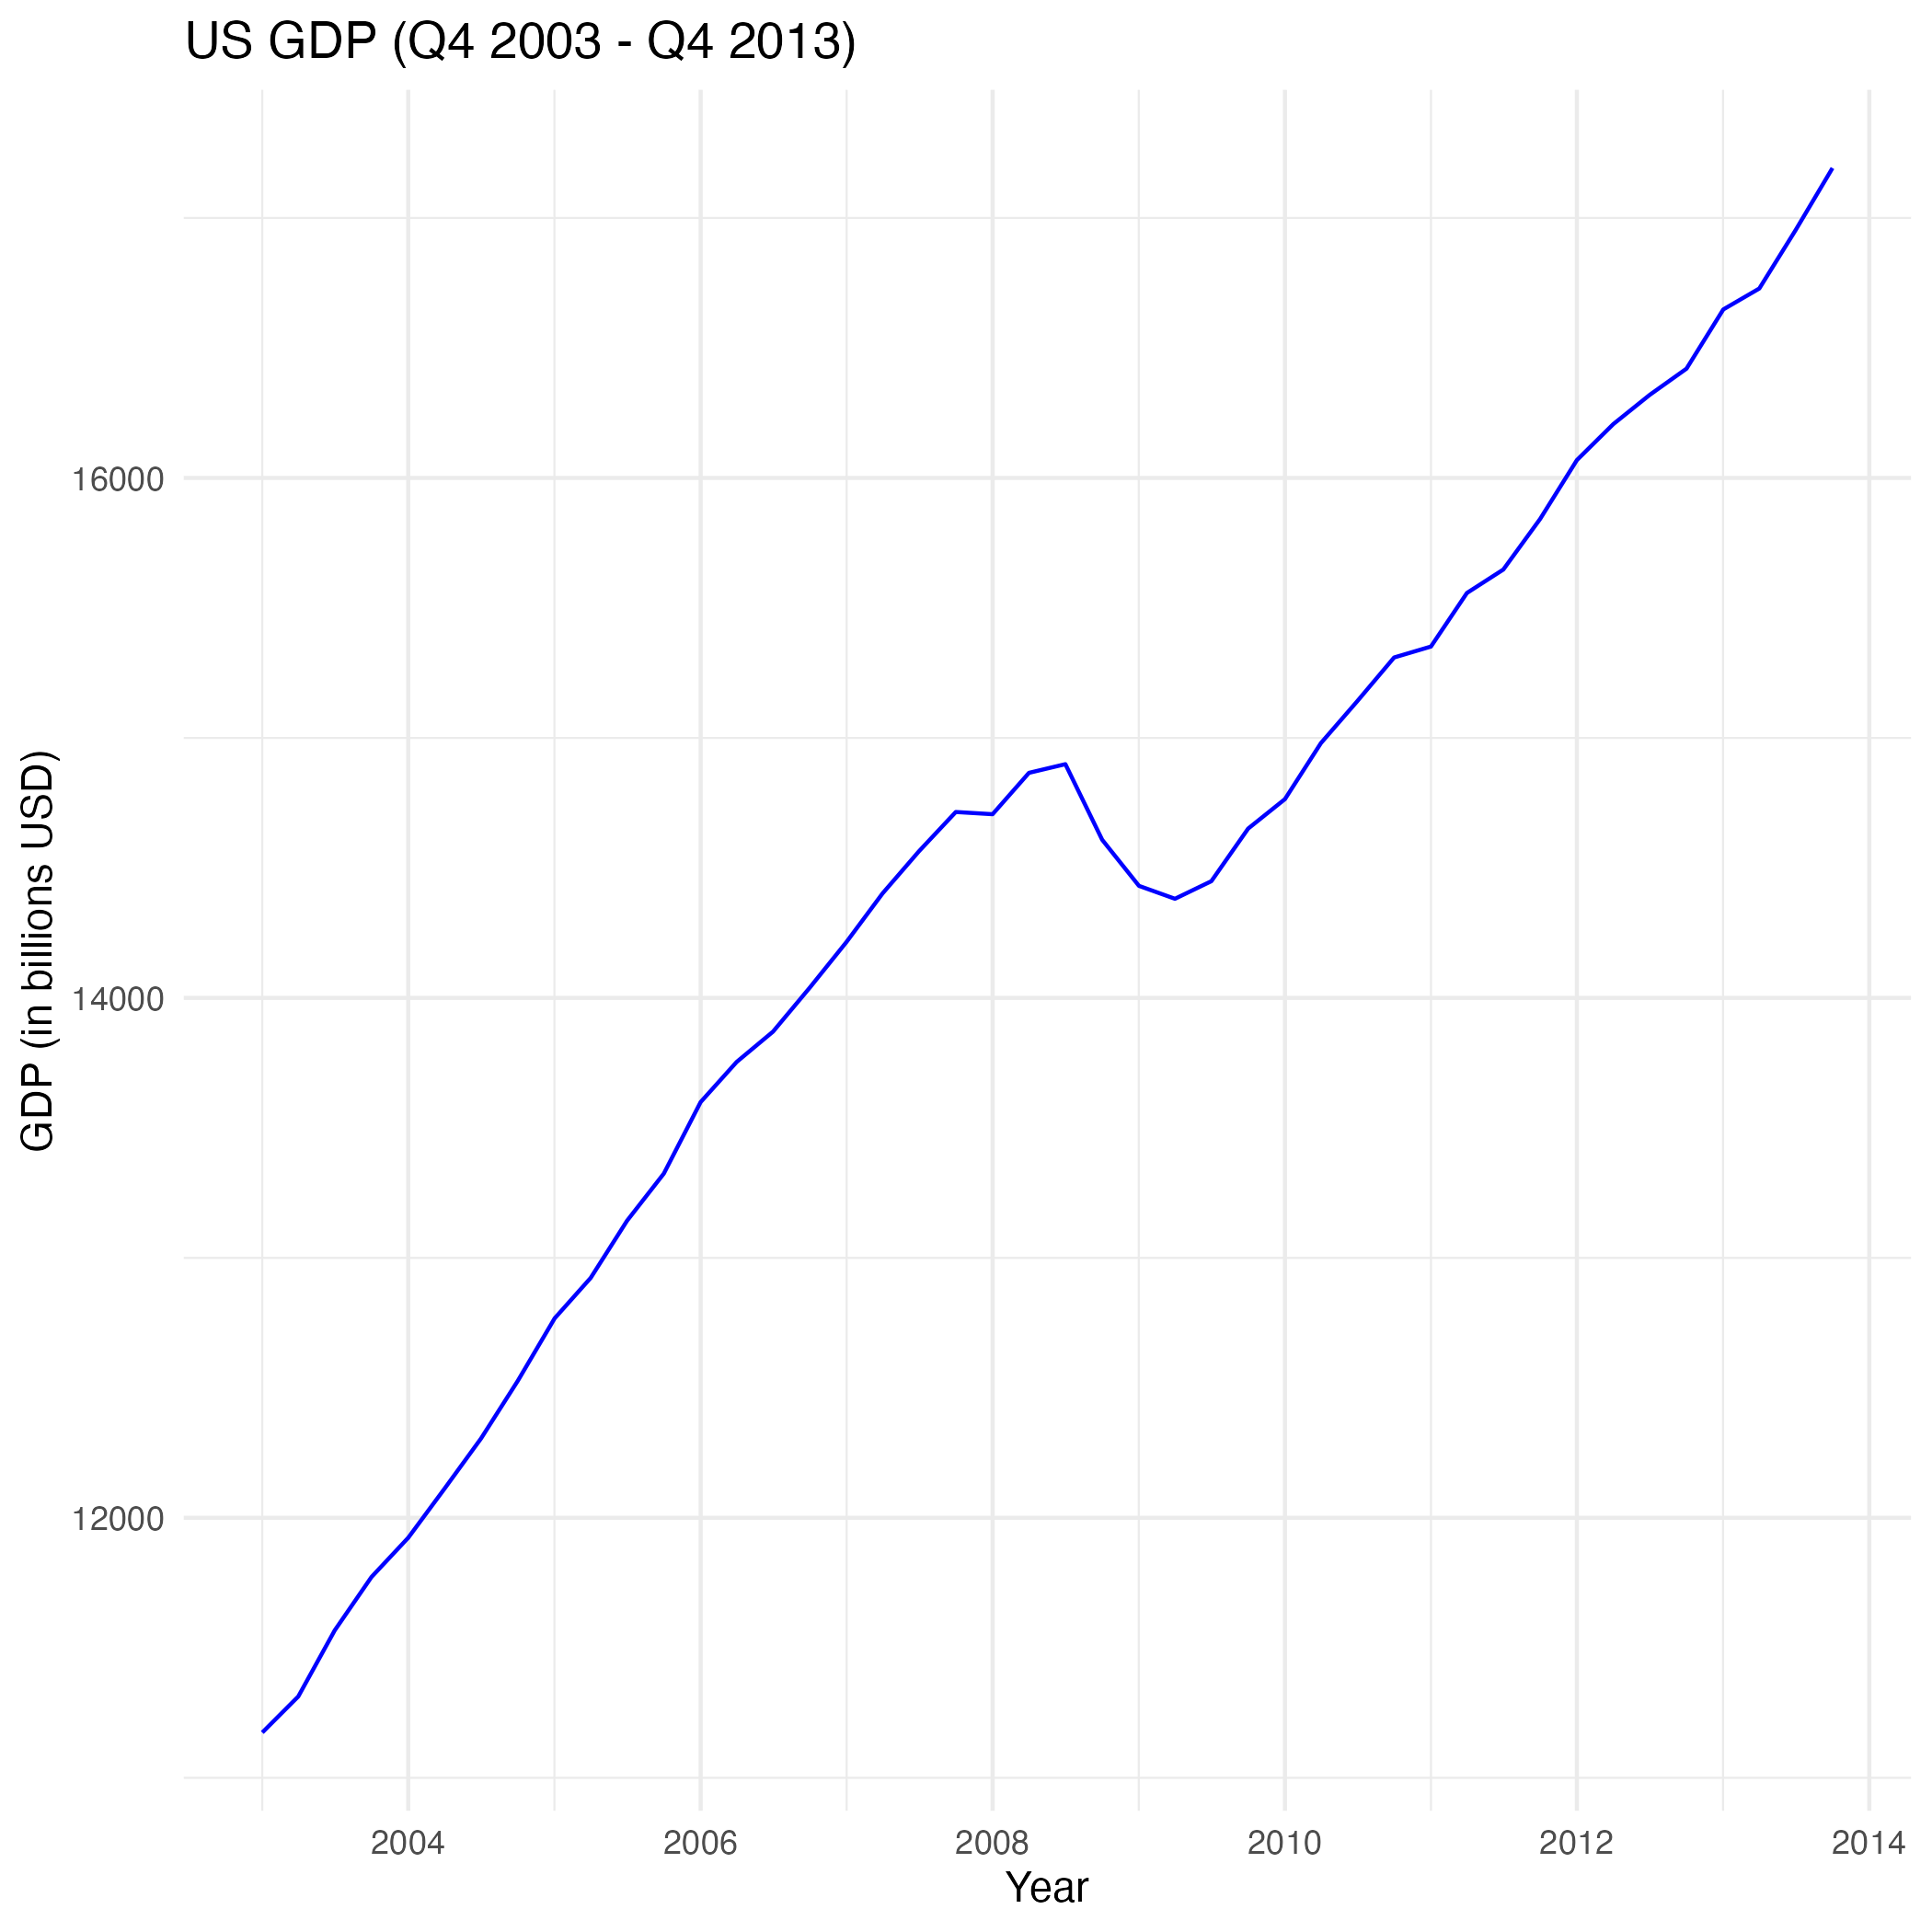
\includegraphics[width=0.8\textwidth]{/Users/cancel/Personal/Coursework/Econ425/FinalWork/R/gdp_graph.png}
    \end{figure}
\end{frame}

\begin{frame}
    \frametitle{Contextual Data --- Inflation}
    \begin{itemize}
        \item Measured by the Consumer Price Index (CPI).
        \item Annual percentage change in cost of a basket of goods and services.
        \item Inflation dropped dramatically, became negative in 2009.
    \end{itemize}
\end{frame}

\begin{frame}
    \frametitle{Graph --- Inflation}
    \begin{figure}[h!]
        \centering
        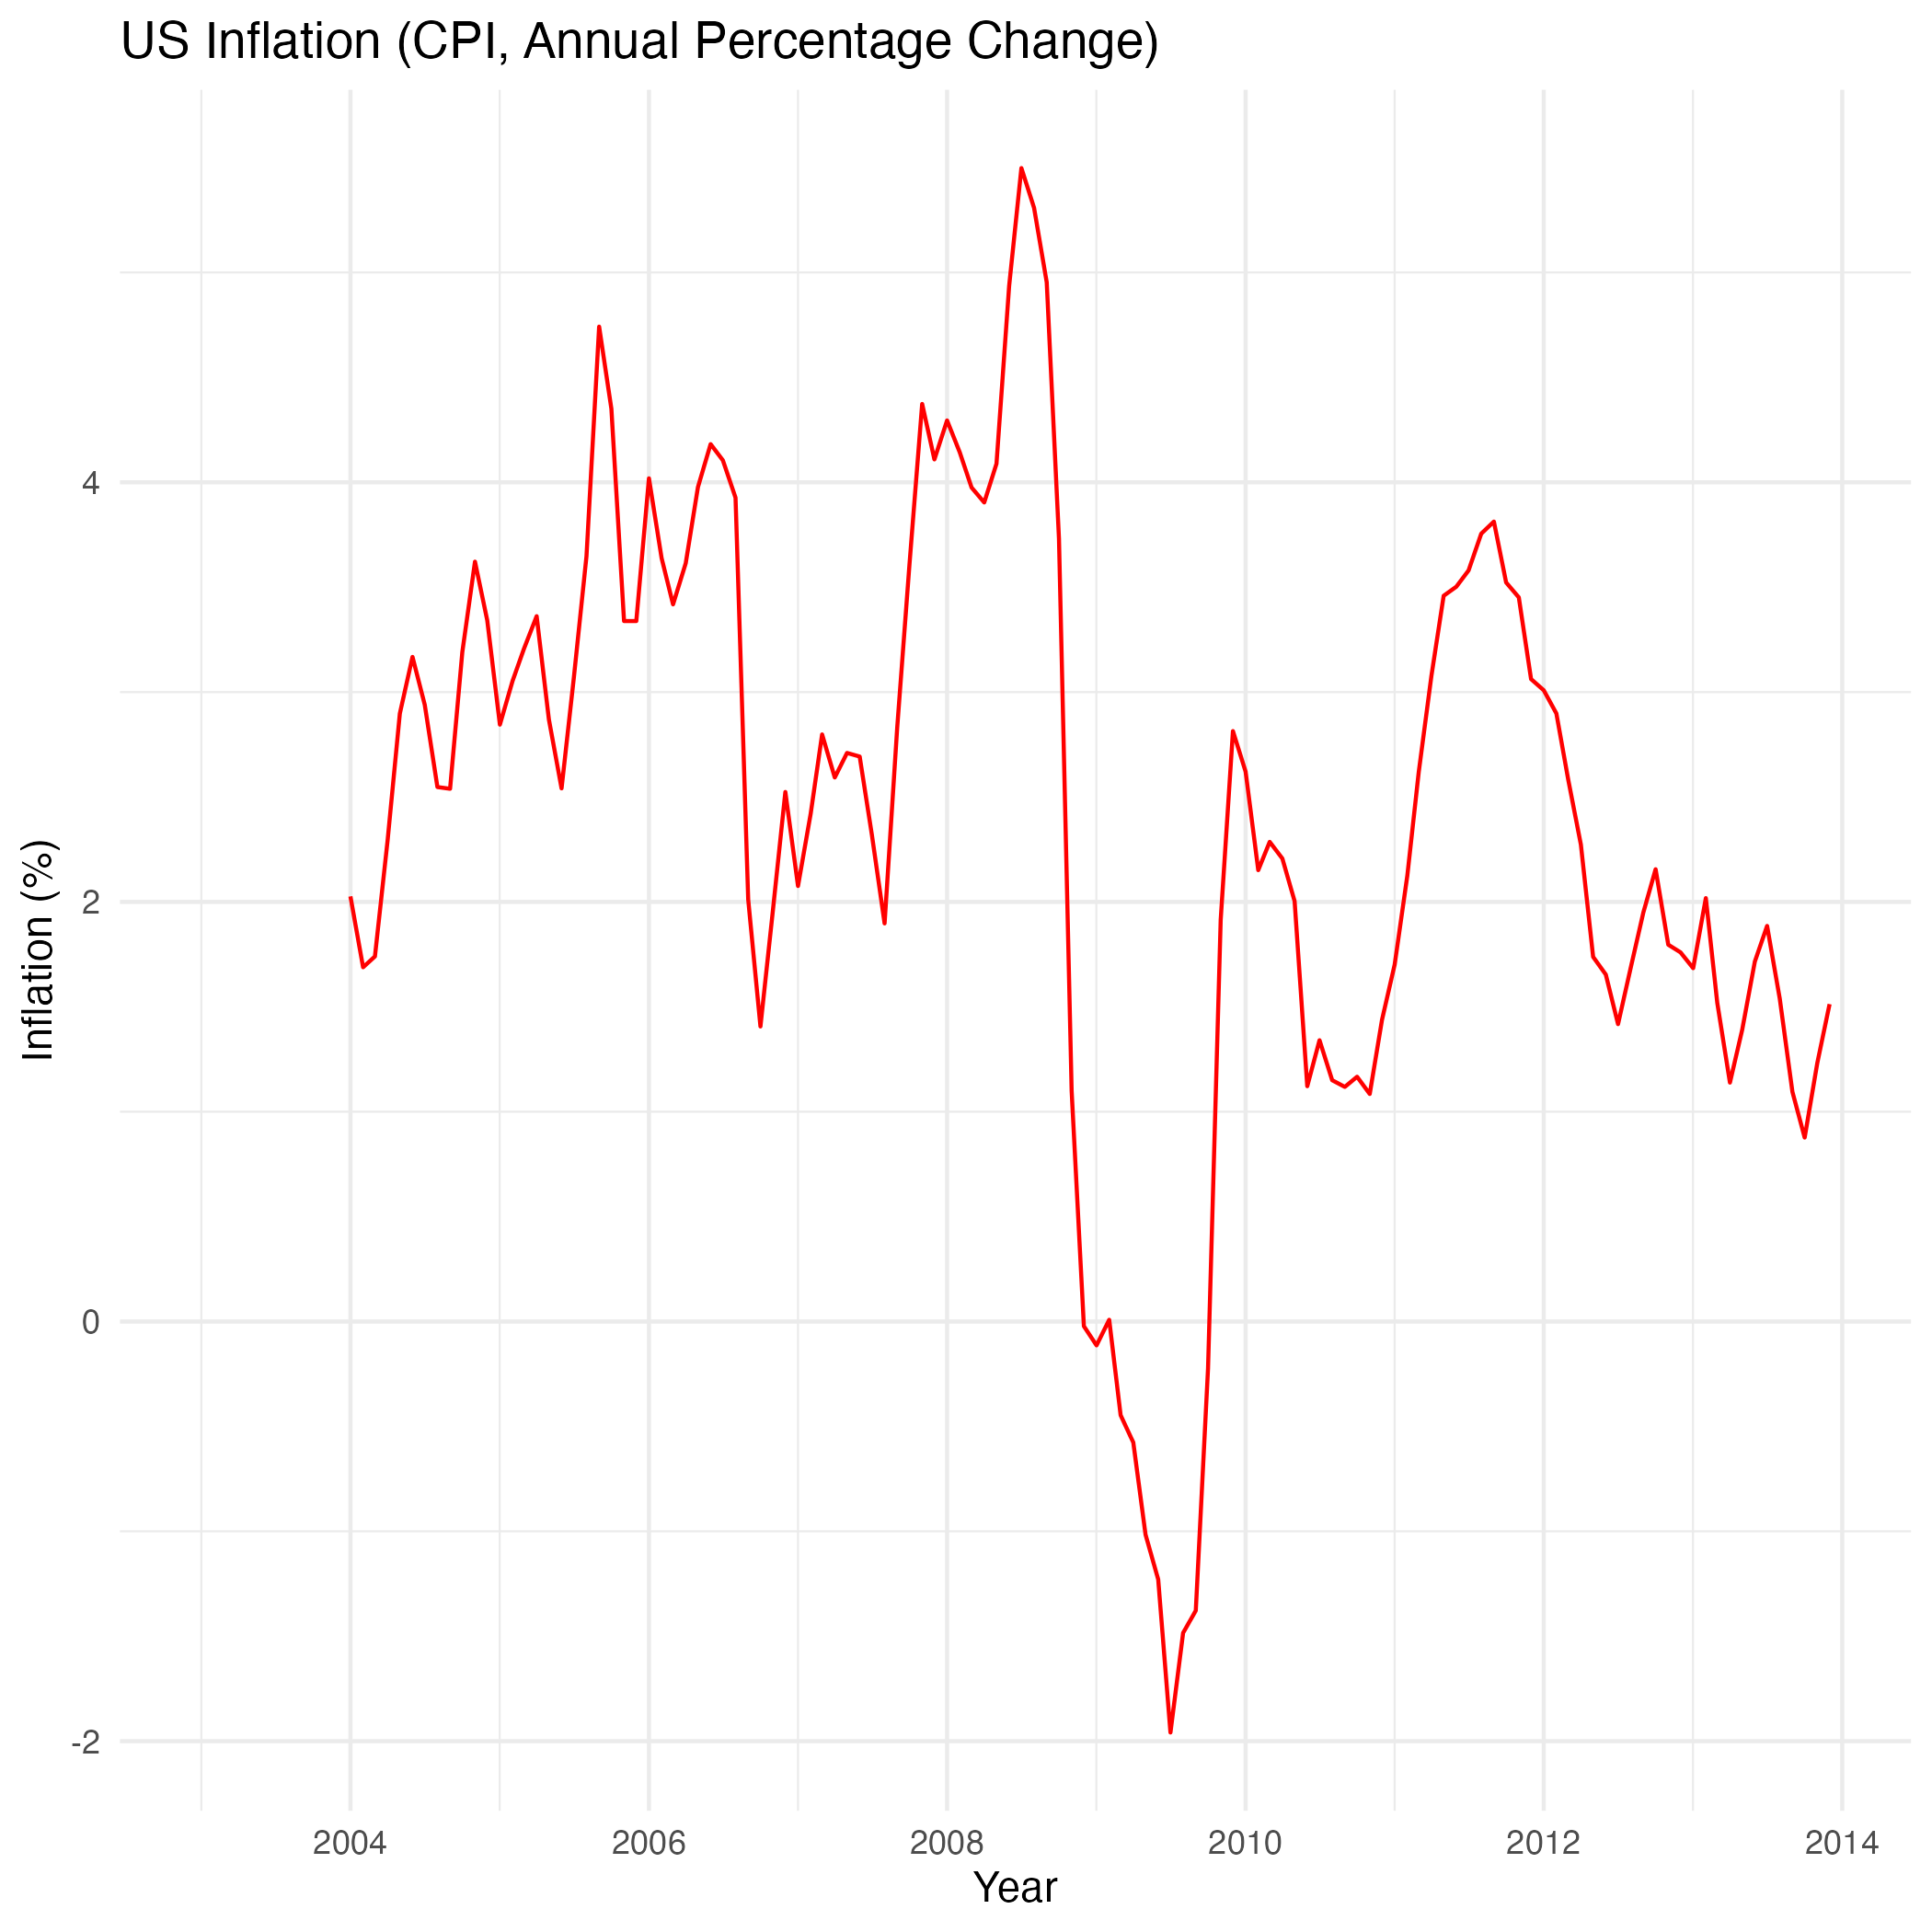
\includegraphics[width=0.8\textwidth]{/Users/cancel/Personal/Coursework/Econ425/FinalWork/R/inflation_graph.png}
    \end{figure}
\end{frame}


\begin{frame}
    \frametitle{Contextual Data --- Interest Rates}
    \begin{itemize}
        \item Federal funds effective rate from 2003 to 2013.
        \item Significant cuts led to extended near-zero rates.
        \item Aimed to stimulate the economy by making borrowing cheaper.
    \end{itemize}
\end{frame}

\begin{frame}
    \frametitle{Graph --- Interest Rates}
    \begin{figure}[h!]
        \centering
        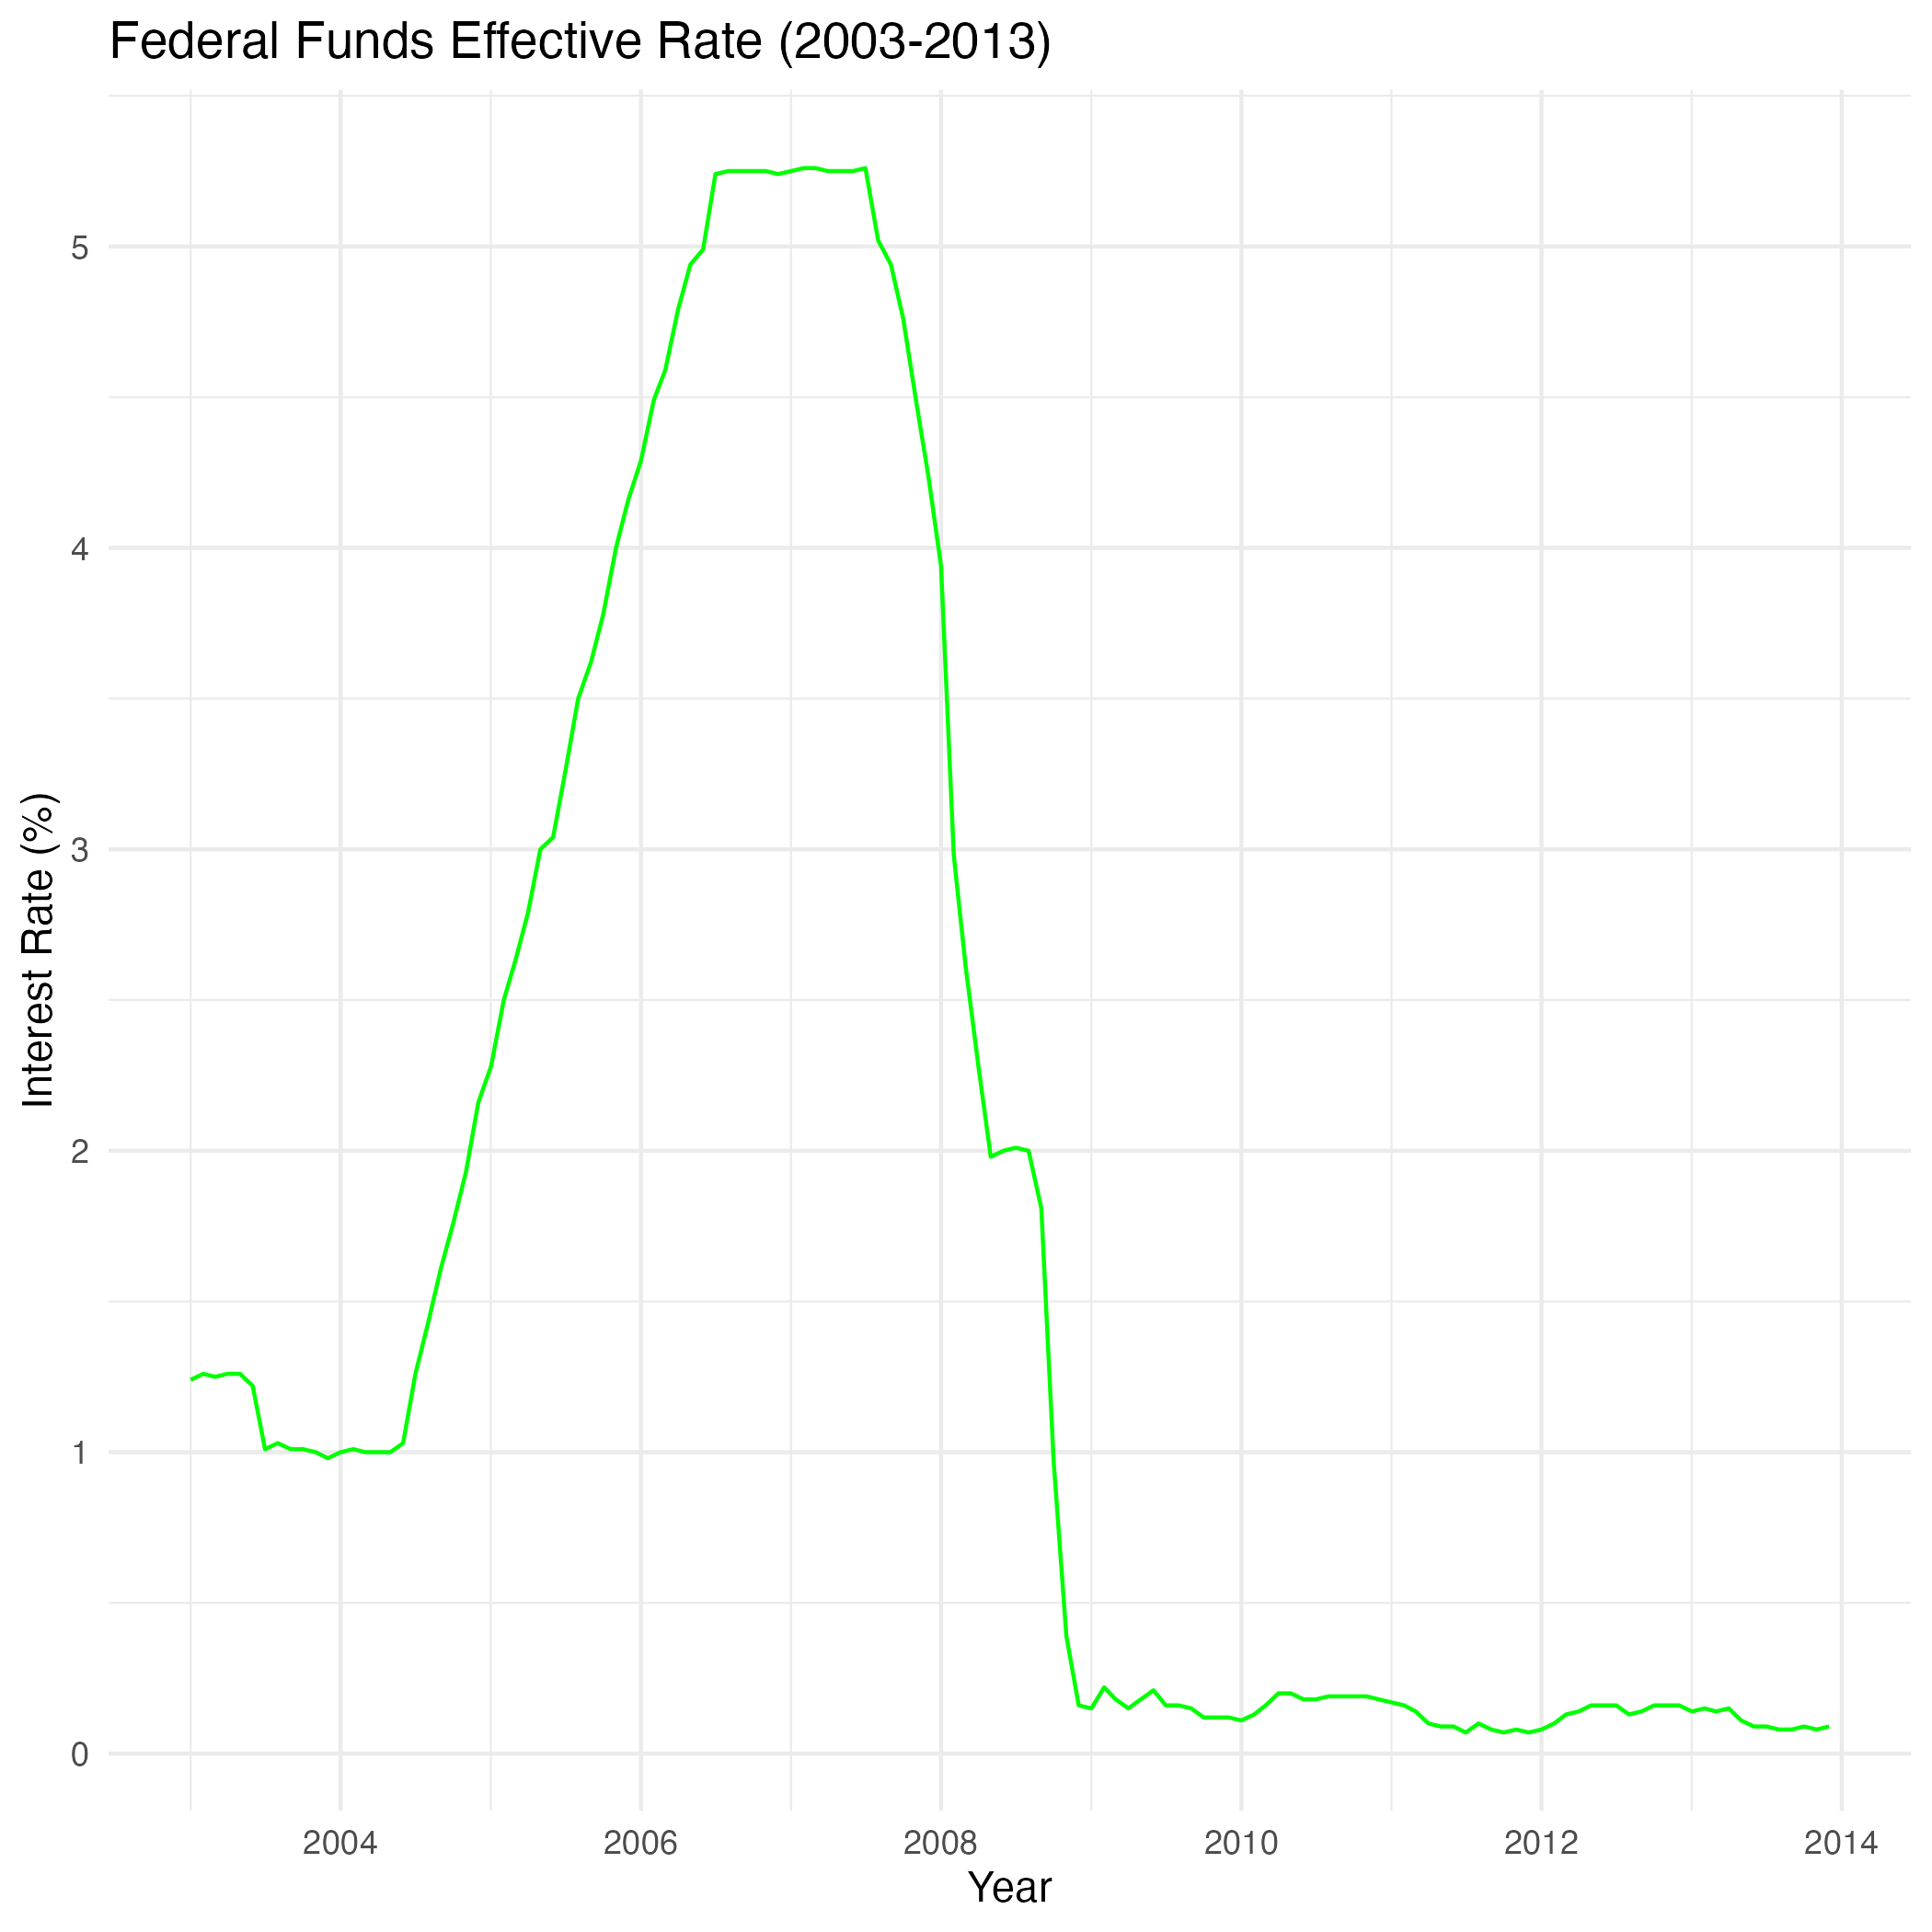
\includegraphics[width=0.8\textwidth]{/Users/cancel/Personal/Coursework/Econ425/FinalWork/R/interest_rate_graph.png}
    \end{figure}
\end{frame}


\begin{frame}
    \frametitle{Contextual Data --- Unemployment Rate}
    \begin{itemize}
        \item Unemployment rate from 2003 to 2013.
        \item Before recession: steady around 5\%.
        \item Peaked at 10\% in October 2009.
    \end{itemize}
\end{frame}

\begin{frame}
    \frametitle{Graph --- Unemployment Rate}
    \begin{figure}[h!]
        \centering
        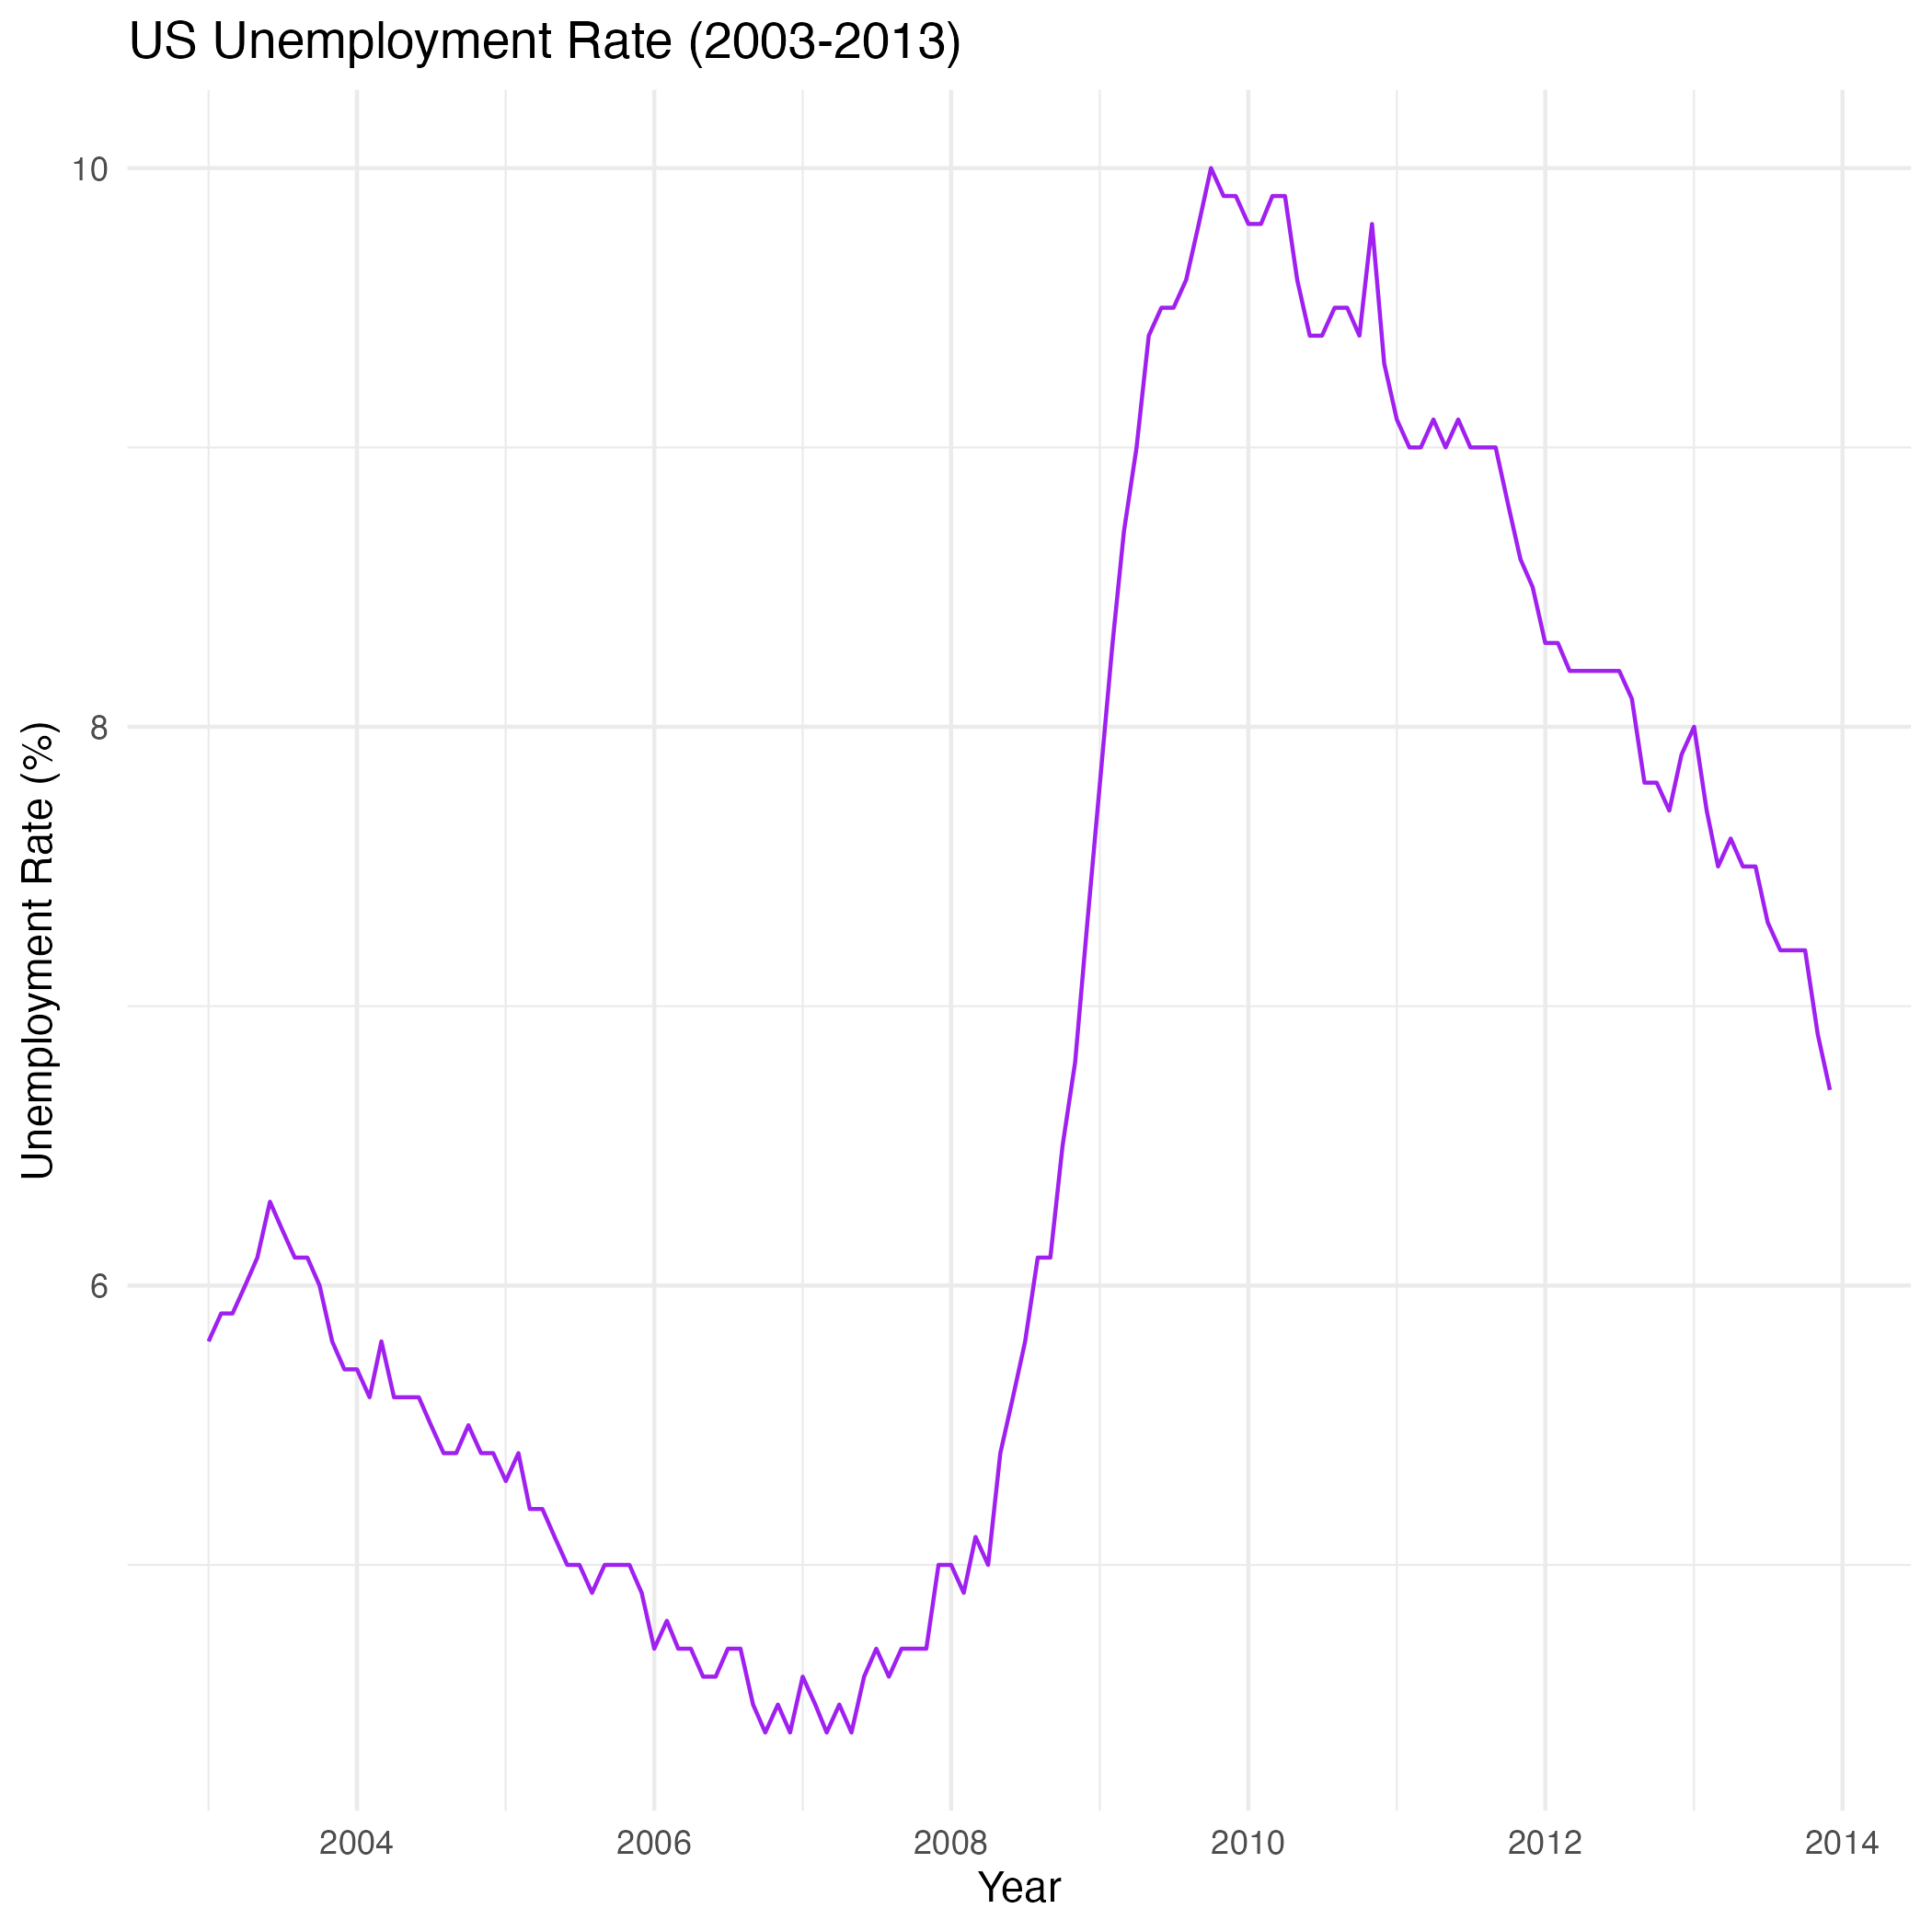
\includegraphics[width=0.8\textwidth]{/Users/cancel/Personal/Coursework/Econ425/FinalWork/R/unemployment_rate_graph.png}
    \end{figure}
\end{frame}

\section{Theory and Decision}
\begin{frame}
    \frametitle{Theory and Decision}
    \begin{itemize}
        \item Crisis: Housing market crisis of 2008 and 2009.
        \item Decision: Lower federal funds rate to around \(0.5\% \pm 0.25\% \).
        \item Rationale: Stimulate spending and investment by making borrowing cheaper.
        \item Aim: Counteract deflationary pressures and support economic recovery.
        \item Consider: Zero interest rate policy and effective forward guidance.
    \end{itemize}
\end{frame}

\section{Statement}
\begin{frame}
    \frametitle{Statement}
    \textit{The Federal Open Market Committee decided today to lower its target for the federal funds rate by 50 basis points to 0.5 percent. Contributing to this decision has been the continued decline of many economic indicators. In particular, a marked deterioration of labor markets and industrial production have led to a bleak outlook. At the same time, prices have continued to decline, and we now project inflation to be at 1 percent for the next couple of years. In spite of this, the Committee believes that the economy will stabilize in the coming year with the implementation of a new stimulus package. The Fed will continue to closely monitor the economy and reaffirms its promise to ensure economic growth and price stability. If necessary, the Fed is willing to further lower the federal funds rate and maintain a lower interest rate for an extended period to reach this goal.}
\end{frame}

\section{Comparison with Fed's Decision}
\begin{frame}
    \frametitle{Comparison with Fed's Decision}
    \begin{itemize}
        \item Fed set a target range of \(0-0.25\%\), more aggressive than our recommended 0.5\%.
        \item Likely aimed for a stronger immediate economic boost.
        \item Implemented extra policies to support mortgage and housing markets and facilitate credit extension.
        \item More aggressive approach likely more effective given worsening economic indicators.
    \end{itemize}
\end{frame}

\section{Conclusions}
\begin{frame}
    \frametitle{Conclusions}
    \begin{itemize}
        \item December 2008 recession: Significant declines in GDP and rises in unemployment.
        \item Our policy: Lower interest rates and provide forward guidance to stimulate economic activity.
        \item Fed's more aggressive approach likely provided a necessary economic boost.
        \item Highlights importance of flexibility and responsiveness in monetary policy during crises.
        \item Future policymakers should consider more aggressive measures in similar situations.
    \end{itemize}
\end{frame}

\section{Q\&A}
\begin{frame}
    \frametitle{Q\&A}
    \begin{itemize}
        \item Thank you for your attention.
        \item This concludes my presentation on the monetary and fiscal policy decisions of December 2008.
        \item I hope this has provided a clear understanding of the economic context and the rationale behind policy decisions.
        \item If you have any questions, please feel free to ask.
    \end{itemize}
\end{frame}

\end{document}
